\documentclass[12pt,a4paper,titlepage,dvipsnames]{article}
\usepackage[a4paper,margin=2cm]{geometry}
\usepackage[utf8]{inputenc}
\usepackage[os=win]{menukeys}
\usepackage{graphicx}
\usepackage{multirow}
\usepackage{tabularx}
\usepackage{wrapfig}
\usepackage{hyperref}


\newcommand*{\appname}{MetGem }
\newcommand*{\appver}{1.0}

\newcommand*{\tsne}{{\em\href{https://en.wikipedia.org/wiki/T-distributed_stochastic_neighbor_embedding}{t-SNE}} }
\newcommand*{\mz}{{\itshape m/z}~}
\newcommand*{\mgf}{\href{http://www.matrixscience.com/help/data_file_help.html}{.mgf} }
\newcommand*{\csv}{\href{https://en.wikipedia.org/wiki/Comma-separated_values}{.csv} }

% inline image with height adapted to text height
\newcommand*{\img}[1]{%
    \raisebox{-.3\baselineskip}{%
        \includegraphics[
        height=\baselineskip,
        keepaspectratio,
        ]{#1}%
    }%
}

% shortcut for centered figure
\newcommand*{\winfig}[1]{%
	\begin{center}
		\includegraphics[scale=0.8]{#1}
	\end{center}
}

% framebox with specified border color
\newcommand{\cfbox}[2]{%
    \colorlet{currentcolor}{.}%
    {\color{#1}%
    \fbox{\color{currentcolor}#2}}%
}

\title{\appname \appver}
\author{Nicolas ELIE  \\
	CNRS / ICSN	}

\begin{document}
\maketitle
\tableofcontents
\newpage

\section{Global Overview}
\begin{center}
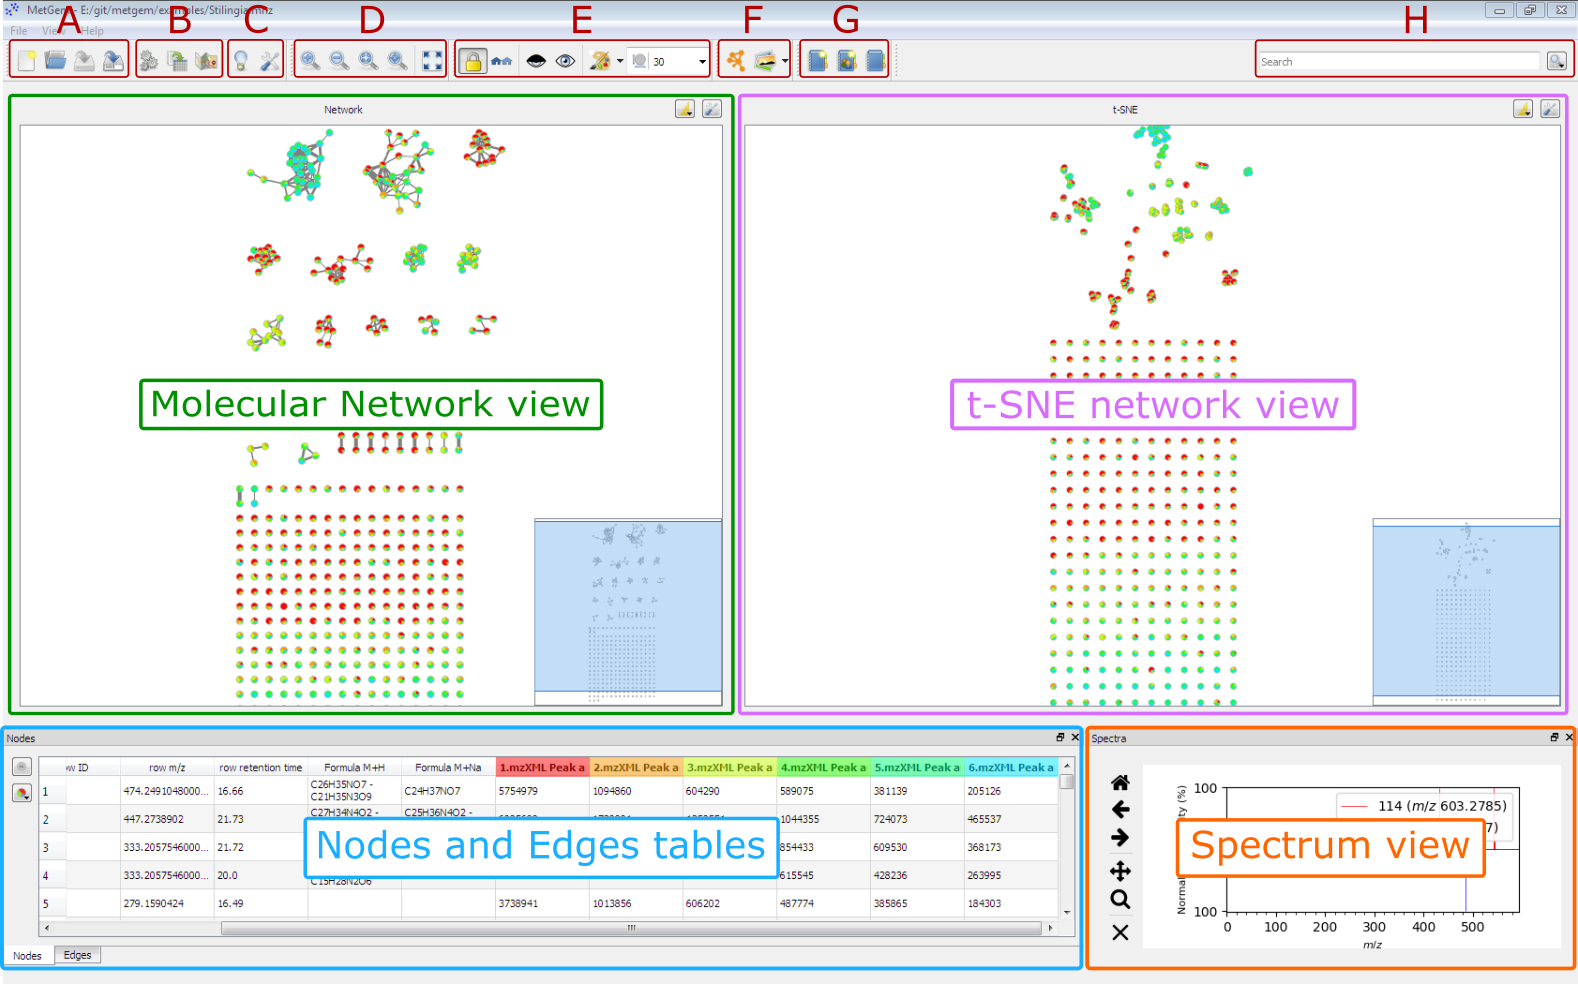
\includegraphics[width=\textwidth]{screenshot1}
\end{center}

\appname's interface is divided is four main parts:
\begin{itemize}
\item Toolbars: See section~\ref{toolbars} on page \pageref{toolbars}.
\item Network Views: See section~\ref{networkviews} on page \pageref{networkviews}.
\item Nodes and Edges tables:  See section~\ref{tables} on page \pageref{tables}.
\item Spectrum View
\end{itemize}

\subsection{Toolbars}
\label{toolbars}
\begin{center}
\begin{tabularx}{\textwidth}{|c|c|X|}
	\hline
	& \bf Name & \bf Description\\
  	\hline
   	A & \multirow{3}{*}{File Toolbar} & Create new project, save/open projects to/from file\\
   	B & & Compute network, load metadata table or load group-mappings \\
   	C & & Show current parameters or change application settings \\
   	\hline
   	D & View Toolbar & Adjust zoom or switch application to fullscreen \\
   	\hline
   	E & Network Toolbar & Link selection between views, select neighbors of selected nodes, hide/show nodes, change selected nodes color/size\\
   	\hline
   	F & Export Toolbar & Export networks to CytoScape or as image\\
   	\hline
   	G & Databases Toolbar & Download, create and explore Databases\\
   	\hline
   	H & Search Toolbar & Search in nodes or edges tables\\
   	\hline
\end{tabularx}
\end{center}

\begin{wrapfigure}[4]{r}{0.25\textwidth}
    \vspace{-.5cm}
	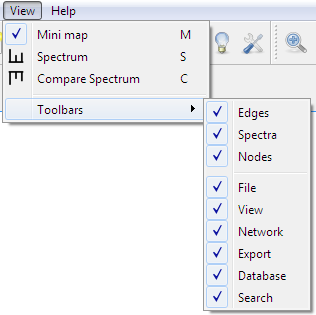
\includegraphics[width=0.23\textwidth]{view-toolbars-menu}
\end{wrapfigure}

Each toolbar can be hidden/shown using the \menu{View > Toolbars} menu. It can also be moved to a different position in the main window or even detached from the latter by simply dragging it to the new position with it's left handle.

\subsection{Network views}
\label{networkviews}
\appname use two different views:
\begin{itemize}
	\item On the left, a classical Molecular Network view like what can be obtained by the \href{https://gnps.ucsd.edu}{GNPS platform}. In this view, each node represent an MS/MS spectrum and each edge represent a the distance between two nodes (obtained via a modified \href{https://en.wikipedia.org/wiki/Cosine_similarity}{cosine-score} calculation). Distance between clusters is arbitrary and has no special meaning.
	\item On the right, a view obtained using \tsne algorithm. This is a 2D projection of the multidimensional space, so no edge is shown but distance between clusters is informative. \tsne algorithm tends to preserve local distances and distort global distances. This means that, if two clusters are close to each other in the original space, they have statiscally more chance than distant clusters to be close in the \tsne projection.\\
	To simplify projection, isolated nodes are excluded from the \tsne processing and are displayed below the \tsne projection. They are arbitrarily distributed and their positions have no special meaning.
\end{itemize}

\begin{wrapfigure}[6]{r}{0.25\textwidth}
    \vspace{-.5cm}
	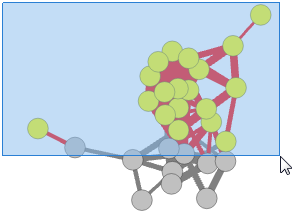
\includegraphics[width=0.23\textwidth]{make-selection}
\end{wrapfigure}

Selection can be done with \img{mouse-left-click} left click on a node/edge or by selecting a region with \img{mouse-right-click} right mouse button. This will automatically filter \hyperref[tables]{metadata tables} to show only metadata from selected nodes/edges (See section~\ref{tables} on page \pageref{tables}).

When a node is selected, the MS/MS spectrum it represents can be loaded in the Spectrum View (See section~\ref{spectrum-view} on page \pageref{spectrum-view}).

You have two options to navigate between network views: either \img{mouse-left-click} click inside a view or use the \keys{\ctrl + \tab} shortcut. Current view will have a \cfbox{cyan}{light blue} outline.

\subsection{Metadata Tables}
\label{tables}
Nodes and edges tables will contains metadata. When nodes or edges are selected in a \hyperref[networkviews]{Network View}, only those nodes/edges will appear in the corresponding tables. Filtering can also be performed using the \hyperref[toolbars]{search toolbar}.

\begin{wrapfigure}[4]{r}{0.25\textwidth}
    \vspace{-1.cm}
	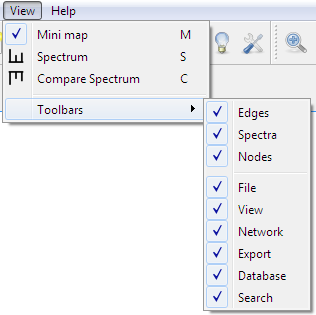
\includegraphics[width=0.23\textwidth]{view-toolbars-menu}
\end{wrapfigure}

These tables can be hidden/shown using the \menu{View > Toolbars} menu. They can also be moved to a different position in the main window or even detached from the latter by simply dragging it to the new position or double-clicking on it's title bar.

\subsection{Spectrum View}
\label{spectrum-view}
The spectrum view is used to visualize nodes' spectra.
\winfig{spectrum-view}

\begin{wrapfigure}[4]{r}{0.25\textwidth}
    \vspace{-.5cm}
	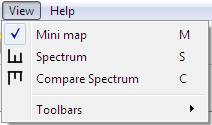
\includegraphics[width=0.23\textwidth]{view-menu}
\end{wrapfigure}

To load a spectrum, simply select a node and use the \menu{View > Spectrum} menu or the \keys{S} shortcut. You can also compare two spectra: select a different node and use the \menu{View > Compare Spectrum} menu or the \keys{C} shortcut. Second spectrum will appear upside-down.

\section{Import data}
\subsection{MGF}
\label{import-mgf}
Networks can be created from a \mgf file using the \emph{\img{process-mgf}Process mgf}~icon. This will open the following dialog:
\winfig{process-mgf-dialog}

This dialog lets you open an \mgf file and, optionally, a metadata table (\csv file) using the \img{browse} buttons. Separator for the \csv file should be auto-detected but you can change this parameter directly in this dialog and more parameters are available via the \img{options} button. See \ref{import-metadata} on page \pageref{import-metadata}.

Parameters used by \appname for the cosine computations step can be tuned  in the \emph{Cosine Score Computing} section.
Parameters for \emph{Network Visualization} and \emph{\tsne Visualization} can be found in their respective sections accessible via the \img{more} button.

When you have loaded an \mgf file and you are satisfied with the parameters, you can click \img{ok} to start the process.

\subsection{Metadata}
\label{import-metadata}
If you have not loaded any metadata during the \hyperref[import-mgf]{\emph{Process mgf}} step or want to load new metadata, you can do so using the \img{import-metadata} tool button from the \hyperref[toolbars]{\emph{File Toolbar}}.
The following dialog will pop-up:
\winfig{import-metadata-dialog}

Metadata file (\csv) can be selected using the \img{browse} button. Separator for \csv file should be auto-detected but can this be changed in the \emph{Options} section. More parameters like whether the file contains headers or not can be also be tuned in this section.

You can see the first 100 lines that will be imported in the \emph{Preview} section. You can select which column to import by clicking on the corresponding headers or via the upper toolbar. If no column is selected, all columns will be imported.

The \img{refresh} button can be used to reload file from disk using the parameters defined in the \emph{Options} section.

\subsection{Group Mappings}

Group mappings file can be used to group columns and sum values they contains. You can load such a file via the \img{import-mapping} tool button.

Group mapping files are simple text files that should follow the following scheme:
\begin{verbatim}
GROUP_group1=filename1.mzXML
GROUP_group2=filename2.mzXML;filename3.mzXML
\end{verbatim}

The example below can be translated as
\begin{quote}
Create a group named \emph{group1} containing columns \emph{filename1.mzXML} and a group \emph{group1} containing columns \emph{filename2.mzXML} and \emph{filename3.mzXML}.
\end{quote}

If a column does not exists, it is simply ignored. Groups can be empty. Group columns are identified with the \img{import-mapping} icon.

\section{Databases}
\subsection{Download}
\subsection{User databases}
\subsection{Explore}
\subsection{Query}

\section{Parameters}
\subsection{Cosine-score computations}
\subsection{Molecular Networking}
\subsection{t-SNE}

\end{document}